\documentclass[12pt]{book}
\usepackage{fontspec}
\setmainfont{TeX Gyre Pagella}
\usepackage[paperwidth=8in,paperheight=8in,margin=0.6in]{geometry}
\usepackage{xcolor}
\usepackage{amssymb}
\usepackage{tikz}
\usetikzlibrary{arrows.meta,shapes.geometric,shapes.misc}
\pagestyle{empty}
\setlength{\parindent}{0pt}

\newcommand{\artnote}[1]{{\color{gray!70}\small\itshape [Illustration: #1]}\par\vspace{0.3in}}
\newcommand{\bigline}[1]{{\Huge #1}\par}
\newcommand{\pagenum}[1]{\vfill{\color{gray!50}\footnotesize #1}}
\newcommand{\sprollpage}{\newpage\vspace*{0.4in}}

\begin{document}

% ============ FRONT COVER ============
\thispagestyle{empty}
\begin{center}
\vspace*{1.1in}
{\Huge \textbf{SPROLL 04}}\\[0.4in]
{\huge \textbf{Not This Way}}\\[0.5in]

\begin{tikzpicture}
\draw[line width=2.5pt] (0,-0.3) rectangle (0.6,0.3);
\draw[line width=2.5pt, red!70] (0,-0.3) -- (0.6,0.3);
\draw[line width=2.5pt, red!70] (0,0.3) -- (0.6,-0.3);
\end{tikzpicture}\\[0.5in]
{\large \textit{a mark that is not an erasure}}\\[0.3in]
{\small The Sproll Curriculum $\cdot$ Cycle I: Pops}
\end{center}

% ============ PAGE 2 ============
\sprollpage
\begin{center}
\vspace*{1.5in}
{\Large The Sproll Curriculum}\\[0.2in]
{\normalsize Cycle I --- Pops: Things, Differences, and Counting}\\[0.6in]
{\small Sproll 04 of 40 \quad $\cdot$ \quad follows Sproll 03: Play It Again}
\end{center}
\pagenum{2}

% ============ PAGE 3 ============
\sprollpage
\begin{center}
\vspace*{0.6in}
\artnote{a field of three shapes: circle bold and chosen, triangle plain, square with a faint line beginning to cross through it}
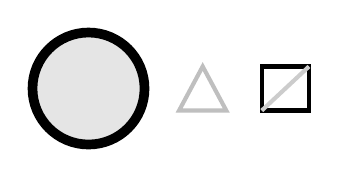
\begin{tikzpicture}
\draw[line width=3.5pt, fill=black!10] (-1.3,0) circle (0.28in);
\draw[line width=1.5pt, gray!50] (-0.15,-0.28) -- (0.15,0.28) -- (0.45,-0.28) -- cycle;
\draw[line width=1.5pt] (0.9,-0.28) rectangle (1.5,0.28);
\draw[line width=1.5pt, gray!40] (0.9,-0.28) -- (1.5,0.28);
\end{tikzpicture}
\vspace{0.35in}
\bigline{Sometimes you say no on purpose.}
\end{center}
\pagenum{3}

% ============ PAGE 4 ============
\sprollpage
\begin{center}
\vspace*{0.7in}
\artnote{the square, clearly crossed out with a bold X, still fully visible beneath the mark}

\begin{tikzpicture}
\draw[line width=2.5pt] (-0.3,-0.3) rectangle (0.3,0.3);
\draw[line width=2.5pt, red!70] (-0.3,-0.3) -- (0.3,0.3);
\draw[line width=2.5pt, red!70] (-0.3,0.3) -- (0.3,-0.3);
\end{tikzpicture}
\vspace{0.35in}
\bigline{Not the square.}
\end{center}
\pagenum{4}

% ============ PAGE 5 ============
\sprollpage
\begin{center}
\vspace*{0.8in}
\artnote{the same crossed-out square, unchanged}

\begin{tikzpicture}
\draw[line width=2.5pt] (-0.3,-0.3) rectangle (0.3,0.3);
\draw[line width=2.5pt, red!70] (-0.3,-0.3) -- (0.3,0.3);
\draw[line width=2.5pt, red!70] (-0.3,0.3) -- (0.3,-0.3);
\end{tikzpicture}
\vspace{0.35in}
\bigline{Is the square gone?}
\end{center}
\pagenum{5}

% ============ PAGE 6 ============
\sprollpage
\begin{center}
\vspace*{0.8in}
\artnote{the crossed-out square again, with a small clarifying note: the shape underneath the X is drawn just as solidly as ever}

\begin{tikzpicture}
\draw[line width=2.5pt] (-0.3,-0.3) rectangle (0.3,0.3);
\draw[line width=2.5pt, red!70] (-0.3,-0.3) -- (0.3,0.3);
\draw[line width=2.5pt, red!70] (-0.3,0.3) -- (0.3,-0.3);
\end{tikzpicture}
\vspace{0.35in}
{\Huge \textbf{No.}}
\end{center}
\pagenum{6}

% ============ PAGE 7 ============
\sprollpage
\begin{center}
\vspace*{0.7in}
\artnote{a small pointing hand or finger, aimed directly at the crossed-out square}
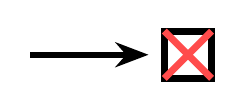
\begin{tikzpicture}
\draw[line width=2.5pt] (0.5,-0.3) rectangle (1.1,0.3);
\draw[line width=2.5pt, red!70] (0.5,-0.3) -- (1.1,0.3);
\draw[line width=2.5pt, red!70] (0.5,0.3) -- (1.1,-0.3);
\draw[-{Stealth}, line width=2pt] (-1.2,0) -- (0.3,0);
\end{tikzpicture}
\vspace{0.35in}
\bigline{You can still point to it.}
\end{center}
\pagenum{7}

% ============ PAGE 8 ============
\sprollpage
\begin{center}
\vspace*{0.4in}
\artnote{a two-line ledger strip: the first line shows a circle labeled Pop, the second line shows a crossed-out square labeled Refuse}
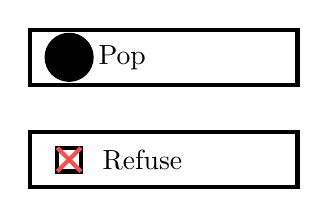
\begin{tikzpicture}
\draw[line width=1.5pt] (-1.7,0.55) rectangle (1.7,1.25);
\filldraw[fill=black] (-1.2,0.9) circle (0.12in);
\node[right] at (-0.95,0.9) {Pop};
\draw[line width=1.5pt] (-1.7,-0.75) rectangle (1.7,-0.05);
\draw[line width=1.5pt] (-1.35,-0.55) rectangle (-1.05,-0.25);
\draw[line width=1.5pt, red!70] (-1.35,-0.55) -- (-1.05,-0.25);
\draw[line width=1.5pt, red!70] (-1.35,-0.25) -- (-1.05,-0.55);
\node[right] at (-0.9,-0.4) {Refuse};
\end{tikzpicture}
\vspace{0.3in}
\bigline{Both are in the record.}
\end{center}
\pagenum{8}

% ============ PAGE 9 ============
\sprollpage
\begin{center}
\vspace*{0.4in}
\artnote{two side-by-side panels: on the left, a completely blank white space with a small question mark, labeled beneath as never chosen and never mentioned; on the right, the crossed-out square, labeled beneath as considered and refused}
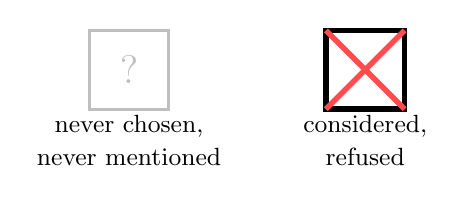
\begin{tikzpicture}
\draw[line width=1pt, gray!50] (-2,-0.5) rectangle (-1,0.5);
\node[gray!50] at (-1.5,0) {\Large ?};
\node[align=center] at (-1.5,-0.9) {\small never chosen,\\\small never mentioned};
\draw[line width=2pt] (1,-0.5) rectangle (2,0.5);
\draw[line width=2pt, red!70] (1,-0.5) -- (2,0.5);
\draw[line width=2pt, red!70] (1,0.5) -- (2,-0.5);
\node[align=center] at (1.5,-0.9) {\small considered,\\\small refused};
\end{tikzpicture}
\vspace{0.55in}
\bigline{These are not the same.}
\end{center}
\pagenum{9}

% ============ PAGE 10 ============
\sprollpage
\begin{center}
\vspace*{0.7in}
\artnote{the crossed-out square once more, calm and simple, no longer needing further contrast}

\begin{tikzpicture}
\draw[line width=2.5pt] (-0.3,-0.3) rectangle (0.3,0.3);
\draw[line width=2.5pt, red!70] (-0.3,-0.3) -- (0.3,0.3);
\draw[line width=2.5pt, red!70] (-0.3,0.3) -- (0.3,-0.3);
\end{tikzpicture}
\vspace{0.35in}
\bigline{Refused is not the same as gone.}
\end{center}
\pagenum{10}

% ============ PAGE 11 ============
\sprollpage
\begin{center}
\vspace*{0.6in}
\artnote{a completely new field: a star chosen and bold, a hexagon plain, a diamond crossed out}
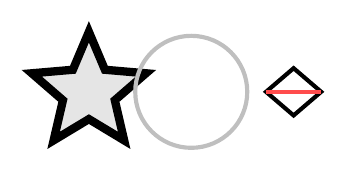
\begin{tikzpicture}
\node[star, star points=5, star point ratio=2.2, minimum size=0.6in, draw, line width=3pt, fill=black!10] at (-1.3,0) {};
\draw[line width=1.5pt, gray!50] (0,0) circle (0.28in);
\draw[line width=1.5pt] (0.95,0) -- (1.3,0.3) -- (1.65,0) -- (1.3,-0.3) -- cycle;
\draw[line width=1.5pt, red!70] (0.95,0) -- (1.65,0);
\end{tikzpicture}
\vspace{0.3in}
\bigline{A new choice. A new refusal.}
\end{center}
\pagenum{11}

% ============ PAGE 12 ============
\sprollpage
\begin{center}
\vspace*{0.5in}
\artnote{the star and the crossed-out diamond, sitting together, both fully visible}
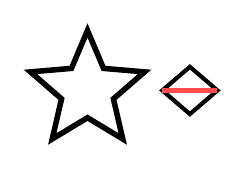
\begin{tikzpicture}
\node[star, star points=5, star point ratio=2.2, minimum size=0.6in, draw, line width=2pt] at (-0.8,0) {};
\draw[line width=1.5pt] (0.15,0) -- (0.5,0.3) -- (0.85,0) -- (0.5,-0.3) -- cycle;
\draw[line width=1.5pt, red!70] (0.15,0) -- (0.85,0);
\end{tikzpicture}
\vspace{0.3in}
\bigline{Same rule. Different shapes.}
\end{center}
\pagenum{12}

% ============ PAGE 13 ============
\sprollpage
\begin{center}
\vspace*{0.6in}
\artnote{a stack of several small ledger strips, each with one Pop line and one Refuse line, suggesting this pattern repeats}
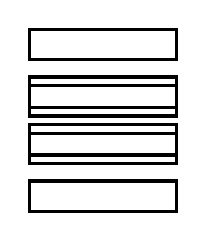
\begin{tikzpicture}[scale=0.55]
\foreach \y in {0,1.1,2.2} {
\draw[line width=1.2pt] (-1.7,0.55+\y) rectangle (1.7,1.25+\y);
\draw[line width=1.2pt] (-1.7,-0.75+\y) rectangle (1.7,-0.05+\y);
}
\end{tikzpicture}
\vspace{0.5in}
\bigline{Every choice can carry its own no.}
\end{center}
\pagenum{13}

% ============ PAGE 14 ============
\sprollpage
\begin{center}
\vspace*{0.8in}
\artnote{the crossed-out square from the very first example, with a small question mark hovering beside it}
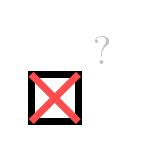
\begin{tikzpicture}
\draw[line width=2.5pt] (-0.3,-0.3) rectangle (0.3,0.3);
\draw[line width=2.5pt, red!70] (-0.3,-0.3) -- (0.3,0.3);
\draw[line width=2.5pt, red!70] (-0.3,0.3) -- (0.3,-0.3);
\node[gray!50] at (0.6,0.6) {\Large ?};
\end{tikzpicture}
\vspace{0.3in}
\bigline{Why keep something you didn't choose?}
\end{center}
\pagenum{14}

% ============ PAGE 15 (closing / hand-off) ============
\sprollpage
\begin{center}
\vspace*{0.5in}
\artnote{a circle and a crossed-out square, with a faint dotted line drawn between them, as if to ask whether they could be connected somehow}
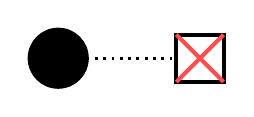
\begin{tikzpicture}
\filldraw[fill=black] (-0.9,0) circle (0.15in);
\draw[line width=1.5pt] (0.6,-0.3) rectangle (1.2,0.3);
\draw[line width=1.5pt, red!70] (0.6,-0.3) -- (1.2,0.3);
\draw[line width=1.5pt, red!70] (0.6,0.3) -- (1.2,-0.3);
\draw[dotted, line width=1pt] (-0.75,0) -- (0.6,0);
\end{tikzpicture}
\vspace{0.35in}
\bigline{Two things happened.}\vspace{0.1in}
{\Large Could they be tied together?}
\vspace{0.4in}\\
{\small \textit{--- turn the page for Sproll 05: Together ---}}
\end{center}
\pagenum{15}

% ============ PAGE 16: Note for Grown-Ups ============
\sprollpage
\vspace*{0.3in}
{\large \textbf{A Note for Grown-Ups}}
\vspace{0.2in}

\normalsize
This book introduces Refuse, the second of the four primitive actions this curriculum builds from. Refusing something is not the same as never mentioning it or erasing it; it is a deliberate act, recorded just as permanently as a Pop, that marks one particular option as not chosen this time, while leaving it fully visible and nameable.

\vspace{0.15in}
Page 9's side-by-side contrast, a blank space that was never mentioned versus a crossed-out shape that was considered and refused, is the entire point of this book stated visually. Confusing the two, treating ``not chosen'' as though it meant ``never existed,'' is a genuinely easy mistake, and this book exists specifically to prevent a child from making it before the idea has a chance to solidify the wrong way.

\vspace{0.15in}
Page 15 closes by asking whether a Pop and a Refuse could be connected to each other. That question is answered, though not resolved completely, in Sproll 05, which introduces the third primitive action, Bind.

\pagenum{16}

\end{document}
